\chapter{Introduction}
\label{ch:intro}

This chapter covers the motivation, contributions and structure of the document.
The main objective of this chapter, therefore, is that after reading it, the reader
forms an idea about the motivations that have promoted this project, what is
being worked on and the contributions emanating from it.

% S E C T I O N   M O T I V A T I O N

\section{Motivation}
\label{sec:intro-motiv}

Each day more and more devices generate data both automatically and manually, and also each day the development of
application in different domains that are backed by databases and expose these data to the web becomes easier. The
amount and diversity of data produced clearly exceeds our capacity to consume it.

To describe the data that is so large and complex that traditional data processing applications can’t handle the
term big-data \cite{big-data,sagiroglu2013big} has emerged. Big data has been described by at least three words starting
by V: volume, velocity, variety. Although volume and velocity are the most visible features, variety is a key concept
which prevents data integration and generates lots of interoperability problems.

In order to solve this key concept RDF \textit{(Resource Description Framework)} was proposed as a graph-based data model
\cite{graph-data-model} which became part of the Semantic Web \cite{semantic-web} vision.
Its reliance on the global nature of URIs\footnote{A Uniform Resource Identifier (URI) is a string of
characters that unambiguously identifies a particular resource. To guarantee uniformity, all URIs follow a predefined
set of syntax rules, but also maintain extensibility through a separately defined hierarchical naming scheme.
Ref.\url{https://en.wikipedia.org/wiki/Uniform_Resource_Identifier}} offered a solution to the data integration
problem as RDF datasets produced by different means can seamlessly be integrated with other data.

Also, and related to this, is the concept of Linked Data \cite{linked-data} that was proposed as a set of best
practices to publish data on the Web. It was introduced by Tim Berners-Lee and was based on four main principles:

\begin{itemize}
  \item Use URIs as names for things.
  \item Use HTTP URIs so that people can look up those names.
  \item When someone looks up a URI, provide useful information, using the standards (RDF, SPARQL).
  \item Include links to other URIs. so that they can discover more things.
\end{itemize}

\begin{figure}
    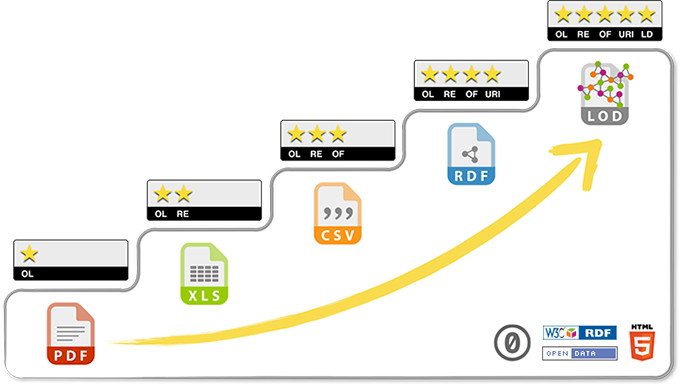
\includegraphics[scale=0.25]{images/5-star-steps.png}
    \centering
	\caption[The 5 star steps of Linked Data]{The 5 star steps of Linked Data.}
	\label{fig:margin-5-star-steps}
\end{figure}

This four principles are called the 5 stars Linked Open Data Model, illustrated in \cref{fig:margin-5-star-steps}.
RDF is mentioned in the third principle as one of the standards that provides useful information. The goal of this
principles is that data is not only ready for humans to navigate through but also for other agents, like computers,
that may automatically process that data.

All the above motivations helped to make RDF the language for the Web of Data, as described in \cite{labra-validating-rdf}.
And the main features that it presents are: \textit{Disambiguation}, \textit{Integration}, \textit{Extensibility}, \textit{Flexibility} and \textit{Open by Default}.
With the features also some drawbacks are associated, the most important one and the one we will focus is the RDF
\textbf{production/consumption dilema}.

RDF production/consumption dilema states that it is necessary to find ways that data producers can generate their data so
it can be handled by potential consumers. For example, they may want to declare that some nodes have some properties with
some specific values. Data consumers need to know that structure to develop applications to consume the data.

Although RDF is a very flexible schema-less language, enterprise and industrial applications may require an extra level of
validation before processing for several reasons like security, performance, etc.

To solve that dilema and as an alternative to expecting the data to have some structure without validation, Shape Expressions Language
\textit{(ShEx)} was proposed as a human-readable and high-level open source language for RDF validation. Initially ShEx was proposed
as a human-readable syntax for OSLC Resource Shapes \cite{oslc-resource-shape} but ShEx grew very fast to embrace more
complex user requirements coming from clinical and library use cases.

Another technology, SPIN, was used for RDF validation, principally in TopQuadrant’s TopBraid Composer. This technology, influenced
from OSLC Resource Shapes as well, evolved into both a private implementation and open source definition of the SHACL
\textit{(Shapes Constraint Language)}, which was adopted by the W3C Data Shapes Working Group.

From a user point of view the possibilities of ShEx are very large, from the smallest case to just validate a node with one property
to a scientific domain case where we need to validate the human genome \textit{(a real use case of ShEx)}. A language with such a number
of possibilities requieres from a strong sintactic and semantic validation and that leads us to our first research question.

\begin{researchquestion}
  How much the existing sintactic and semantic validation systems for shape expressions can be enhanced?
\end{researchquestion}

Secondly and very related to programing languages, if we take the PopularitY of Programming Language \textit{(PYPL)} Index\footnote{\url{http://pypl.github.io/PYPL.html}}
from June 2020 we can see that more than half of the share is occupied by languages that support the object orienten paradigm. And therefore this paradigm
becomes the most used one. The aim of this paradigm is to model real world domains, acocrding to \cite{wegner1990concepts}. That, in fact, is the same goal
that ShEx has, it allows to model real world domains with schemas, and validate existing data with them. Therefore our second research question relies on this and tries
to automatically transform shape expressions into object domain models coded in any language that supports the object oriented paradigm:

\begin{researchquestion}
  Till which point can we automatically translate existing shape expressions in to object domain models?
\end{researchquestion}

If this were possible it would not only imply that you could automate the creation of application domain models but that you could link the domain model that an
application uses with a domain model defined through Shape Expressions that describes the schema of a RDF data set.

\bigskip

To give answers to the questions posed in this section, we will limit our scope to the micro grammar of Shape Expressions, defined in
\footnote{\url{https://dcmi.github.io/dcap/shex_lite/micro-spec.html}}. This version is a strict subset of the complete ShEx grammar
and therefore any conclusion we can draw from it can automatically be applied to the full grammar.

% S E C T I O N   C O N T R I B U T I O N S

\section{Contributions}
\label{sec:intro-contri}
These are the major contributions of this dissertation:

\begin{enumerate}
  \item A parser for the ShEx micro Compact Syntax. There are already existing parsers for ShEx and they work for ShEx micro Compact Syntax
  as it is a subset of ShEx, but they accept more structures than the ones defined by ShEx micro Compact Syntax. We propose a parser that
  is only focused on ShEx micro Compact Syntax and therefore error and warning messages can be enhanced.
  
  \item Error and warning analyzer for schemas. Existing approaches do not semantically validate the schemas, they
  only perform error detection by means of complex grammars and parsers. Our proposed system does semantically validate the schemas by means
  of a custom analyzer that performs both sintactic and semantic analysis so it produces human-friendly errors and warnings that users can
  use to fix their schemas.

  \item Automatic translation of schemas in to object domain models in \texttt{Java} and \texttt{Python}. The proposed system
  integrates an open back-end with build-in code translation from the validated schemas to domain models in object
  oriented programming languages \textit{(OOPL)} \cite{oopl}.

  \item Evaluation of errors and warning generated of our proposed soulution against existing tools. This comparison
  empirically shows the benefits and drawbacks of our proposed system.
\end{enumerate}

% S E C T I O N   S T R U C T U R E   O F   T H E   D O C U M E N T

\section{Structure of the Document}
\label{sec:intro-structure}
The dissertation layout is as follows:
\bigskip

\begin{description}
  \item[\cref{ch:theo-back}] Indicates the state of the art of the existing RDF validation technologies, tools for processing Shape
  Expressions and other related projects.
	\item[\cref{ch:retalted-work}] Gives a basic theoretical background that it is needed to fully understand the concepts explained in the
  following chapters.
  \item[\cref{ch:proposed-system}] Contains a detailed initial planning and budget for the project, this is the designed planning followed
  during the execution of the project and the initial estimated budget.
  \item[\cref{ch:results-evaluation}] Gives a basic theoretical background that it is needed to fully understand the concepts explained in the
  following chapters.
  \item[\cref{ch:planning-and-budget}] Provides a technical description of the design and implementation of the compiler itself. This includes,
  analysis, design, the technological stack choices, diagrams, implementation decisions and tests.
  \item[\cref{ch:conclusions}] Compares the initial planning developed in chapter 4 with the final one. This includes the genuine execution
  planning of the project and the reasons and events that modified the one from chapter 4.
\end{description}